
\section{System Model}
\label{sec:model}

In this section, we present our model for transactions, invariants,
and coordination.

\minihead{Databases} In this paper, we consider a set of users
accessing a shared database, which contains a \textit{versioned} set
of data items. In our initial formulation, we will represent database
state as a bag of mutations (much like a write-ahead
log~\cite{gray-book}), but we will consider other, more pragmatic
representations in Section~\ref{sec:bcc-practice}. The database is
initially populated by an initial state $D_0$ (typically but not
necessarily empty), and copies of database state can be combined via a
``merge'' operator ($\sqcup$: $DB \times DB \rightarrow DB$).  For
simplicity, we require merge to be commutative, associative, and
idempotent~\cite{calm,crdt}. In our ``bag of mutations'' model, merge
is simple set union, but we will consider alternative implementations
in Section~\ref{sec:bcc-practice}.

\minihead{Transactions} Users submit requests to the database in the
form of transactions, or groups of operations on data items that
should be executed together: we define a transaction $T$ as a
transformation on state: $T: DB \rightarrow DB$. Individual operations
are often in the form of writes (which add new versions to the
database) or reads (which return a specific set of versions from the
database), but operations can also operate on abstract data types,
such as incrementing a counter item or adding an item to a set
item. When required---and certainly in later sections of this
paper---we will discuss specific operation types, but, in general, we
will not make any specific assumptions about operations. A transaction
can \textit{commit}, signaling success, or \textit{abort}, signaling
failure. In our model, effects of aborted transactiosn will not be
reflected in database state (i.e., aborted writes will be rolled
back). This provides Read Committed isolation and does not affect our
results (e.g., is achievable with availability by waiting to write
until commit time~\cite{hat-vldb,spanner}).

\minihead{Invariants} As we have discussed, users accessing a shared
database have notions of correctness, which we capture in our system
model via \textit{invariants}. In our model, users specify invariants
over arbitrary database state that determine whether a given state is
valid according to application rules. We model invariants as binary
predicates on database state: $I: DB \rightarrow \{true, false\}$.  As
an example, an invariant might express the requirement that only one
user in a database has a given ID. This directly captures the notion
of ACID Consistency~\cite{bernstein-book,gray-virtues}, and we say
that a database state is \textit{valid} under an invariant $I$ (or
$I$-valid) if it satisfies the predicate:

\begin{definition}
A database state $D$ is \textit{valid} under $I_s$ if $I_s(D) \rightarrow true$.
\end{definition}

We wish to analyze sequences of valid transactions that transitively
maintain validity of database state, so we require that $D_0$ be valid
under declared constraints.

\miniheadnostop{Why specify invariants?} Much of the existing work on
database concurrency control assumes a model whereby ``the [set of
  invariants] is generally not known to the system but is embodied in
the structure of the transaction''~\cite{traiger-tods}. Indeed,
Eswaran et al.'s seminal paper on the topic of consistency argues that
``a complete set of assertions would no doubt be as large as the
system itself''~\cite{eswaran-consistency}. Nevertheless, since 1976,
databases have introduced support for a finite set of
invariants~\cite{korth-serializability} in the form of primary key and
foreign key, uniqueness, and row-level ``check'' constraints. We
expand this set of invariants in Section~\ref{sec:bcc-practice} and
demonstrate that a small set of invariants provides expressive power
for many applications. It is possible to perform a conservative
analysis if a complete specification of invariants is missing, but
this will result in less useful results. Unlike more general forms of
axiomatic logic (e.g., Hoare-style triples~\cite{decomp-semantics}),
we require only one set of invariants per application.\vspace{.5em}

\minihead{Replicas} In this paper, we are concerned with
synchronization and coordination between multiple transactions. To
begin, we consider a system model with multiple copies of database
state (\textit{replicas}) that can each respond to transaction
requests (we do not further distinguish between partitioned and
fully-replicated replicas~\cite{hat-vldb} as our results do not
require it). While most treatments of database systems treat replicas
as individual servers, a single-site (or mastered) database can also
provide users with an interface that exposes multiple ``replicas''. A
multi-versioned database system~\cite{bernstein-book} effectively
provides each user with a logical replica of database state that is
isolated from concurrent access and modification. A set of invariants
and stored procedures that are executable without coordination in a
distributed context can also be executed in parallel on a single-site
system without stalling due to concurrent operations.  In fact, our
current prototype transaction model (Section~\ref{sec:evaluation}) is
based on multi-versioning and snapshot reads (``logical replicas'')
rather than physical multi-master replication. Accordingly, we assume
that, if a client can access a physical server responsible for a given
data item, it can access a replica for the item without
blocking. Therefore, all concurrent operations will behave as if they
are executed on separate replicas.

\minihead{Availability} To reflect the requirement that each user's
transactions eventually receive a response, we need a definition of
\textit{availability}. To prevent the system from simply aborting
transactions (which guarantees a response---albeit a not very useful
one), we adopt the following definition of
availability\footnote{As Bailis et
  al. note~\cite{hat-vldb}, this definition precludes multi-server
  fault tolerance (durability). However, we can consider multi-server
  durability by extending this definition to include coordination with
  a (typically small~\cite{bigtable,spanner,dynamo}) fixed number of
  servers. This does not greatly affect scalability because, as more
  replicas are added, durability-related communication is constant.}~\cite{hat-vldb}:

\begin{definition} 
A system provides \textit{transactional availability} if, whenever a
client executing a transaction $T$ can access at least one replica for
each item in $T$, $T$ eventually commits or otherwise aborts itself
either due to an \textit{abort} operation in $T$ or if committing the
transaction would violate a declared invariant over replica state.
\end{definition}

According to the above definition, a transaction can only abort if it
explicitly chooses to abort itself (e.g., a given item does not exist
in a warehouse) or if the effects of the transaction would invalidate
the replica state.

\minihead{Convergence} Transactional availability allows replicas to
maintain valid state \textit{independently} but, without additional
constraints, it is vacuously possible to maintain ``consistent''
database states by letting replicas diverge forever. For example,
replicas $R_i$ and $R_j$ might each contain valid state but their
combined contents may not be valid (e.g., a user $u_i$ on $R_i$ is
assigned id $5$ and a separate user $u_j$ on $R_j$ is assigned the
same ID, satisfying the invariant that user IDs are unique locally but
not globally). In distributed systems parlance, this guarantees
\textit{safety} (nothing bad happens) but not \textit{liveness}
(something good happens)~\cite{lamport-safety}. To ensure that
replicas eventually agree---reflecting a shared, common set of
database state---we adopt the following definition:

\begin{definition}A system is \textit{convergent} if, in the
absence of new transactions and in the absence of indefinite
communication delays, all replicas eventually contain the same state.
\end{definition}

This convergence, or \textit{eventual consistency}, requirement forces
replicas to exchange state at some point in the future (i.e., via
\textit{anti-entropy} processes)~\cite{vogels-defs}. To capture the
process of reconciling divergent copies of database state, we use the
previously discussed merge operator: given two copies of divergent
database state, replicas apply the merge operator to produce a single
copy of database state. Our intial formulation of merge as a simple
set union makes reconciliation simple, but, again, we will discuss
alternative merge operators in Section~\ref{sec:merge}. Importantly,
convergence can occur as an \textit{asynchronous} (i.e., background)
process and can safely stall at any point given that---at some point
in the future---merging occurs.

\minihead{Maintaining validity} A transactionally available system
that does not communicate can maintain consistency on a per-replica
(or set of replica basis), but, once the replicas converge, we have no
guarantee of per-replica consistency. In the example above, once $R_1$
and $R_2$ merge their divergent states, their converged state will be
invalid. Our choice of convergence via union-based merge requires that
$R_1$ and $R_2$ cannot simply ``throw away'' writes (i.e., tentative
updates~\cite{tamer-book}) to ensure consistency (again, a deliberate
choice that we will revisit in Section~\ref{sec:merge}). To capture
the requirement that replica states are valid not only during
operation but also after merge, we introduce the following definition:

\begin{definition}
A system is \textit{globally $I$-valid} if all replicas always contain
$I$-valid state.
\end{definition}

\minihead{Coordination} A transactionally available, globally valid,
convergent system provides a guaranteed response, maintains replica
validity, and ensures that replicas agree. However, our system model
is missing one final constraint: coordination between
replicas. Indeed, with network failures, a transactionally available
system will provide responses without synchronous communication
between replicas. However, in the absence of (or given a network model
that does not consider) network failures (i.e., an omission model), a
system satisfying the above three properties can still coordinate
between replicas, potentially compromising scalability. To rule out
the possibility of coordination under both scenarios, we adopt the
following definition of coordination-freedom:

\begin{definition}
A system is \textit{\cfree} if replicas do not communicate in order to
execute transactions.
\end{definition}

Figure~\ref{fig:replicas} illustrates a coordination-free execution of
two transactions $T_1$ and $T_2$ on two separate replicas of
(complete) database state. Each transaction commits on its local
replica, which subsequently forwards the new database state to the
other replica in the background. By applying the merge operator of set
union, each replica contains the same database state.

\begin{figure}
\begin{center}
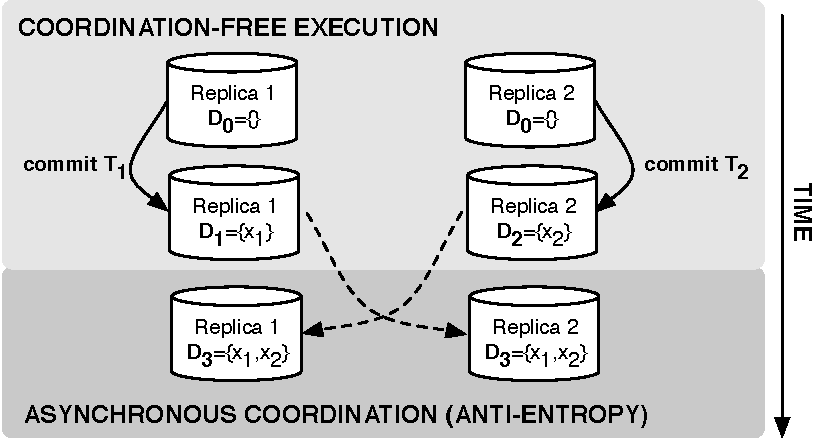
\includegraphics[width=.85\columnwidth]{figs/replicas.pdf}
\end{center}\vspace{-1em}
\caption{An example coordination-free execution of two transactions,
  $T_1$ and $T_2$ on two replicas of database state. Each transaction
  commits on a replica, then, after commit, the replicas exchange
  their new writes asynchronously and converge on a common database
  state ($D_3$).}
\label{fig:replicas}
\end{figure}


\begin{table}
\begin{center}
\small
\begin{tabular}{|l|r|}
\hline\textbf{Requirement} & \textbf{Effect}  \\\hline
Global validity & Invariants are never violated \\
Transactional availability & Non-trivial response guaranteed \\
Convergence & Replicas must reconcile \\
Coordination-freedom & No synchronous coordination\\\hline
\end{tabular}
\end{center}\vspace{-1em}
\caption{Utility of requirements in system model.}
\label{table:requirements}
\end{table}


\minihead{Summary} A globally valid, transactionally available,
convergent, and \cfree system achieves our intended goals of perfect
scalability, availability, and low latency. As we summarize in
Table~\ref{table:requirements}, every copy of database state is valid
with respect to invariants, each transaction receives a non-trivial
response, database states eventually agree, and all transactions are
processed without communication. The above definitions---while
somewhat pedagogical---rule out trivial implementations that satisfy
our informal goals but compromise ``useful'' behavior. Using this
formalism, we can subsequently understand when these goals are
achievable.
